% -------------------------------------------------------------------
\RequirePackage{fix-cm}
\documentclass[12pt,a4paper,twoside]{article}

\usepackage{graphicx,xcolor,textpos}
\usepackage{helvet}
\usepackage{amsmath}
\usepackage{rotating}
\usepackage{amsfonts}
\usepackage{amssymb}
\usepackage{graphicx}
\usepackage{tikz}
\usepackage{pdflscape}
\usepackage[section]{placeins}
\usepackage{afterpage}
\usepackage{capt-of}% or use the larger `caption` package
\usepackage{enumitem}
\usepackage{caption}
\usepackage{subcaption}

\usepackage{aas_macros}
\usepackage{natbib}

\newcommand\encircle[1]{%
  \tikz[baseline=(X.base)] 
    \node (X) [draw, shape=circle, inner sep=0] {\strut #1};}
\newcommand{\Alfven}{Alfv\'{e}n } 
\newcommand{\Alfvenic}{Alfv\'{e}nic }

% ------------------------ Page settings -----------------------------
% If you change these, the cover layout will also change.  In that
% case you have to adjust the latter manually.
% --------------------------------------------------------------------

\topmargin -10mm
\textwidth 160truemm
\textheight 240truemm
\oddsidemargin 0mm
\evensidemargin 0mm

\begin{document}
\begin{titlepage}
	\centering
	
\includegraphics[width=0.5\textwidth]{logo_uni2.jpg}\par\vspace{1cm}
	{\scshape\LARGE The University of Sheffield \par}
	\vspace{1cm}
	{\scshape\Large Literature Review\par}
	\vspace{1.5cm}
	{\Large\bfseries Numerical MHD Investigation of the Microphysics in the Solar Atmosphere\par}
	\vspace{2cm}
	{\Large\itshape Fionnlagh Mackenzie Dover\par}
	\vfill
	\large supervised by\par
	\Large Prof.~ R\'{o}bert Erd\'{e}lyi

	\vfill

% Bottom of the page
%	{\large \today\par}
\end{titlepage}
\setcounter{page}{0}
\section*{List of Symbols}
Below is a list of the notation used throughout the text unless stated otherwise: \\ \\
$\rho$ $\rightarrow$ Density.  \\
$p$ $\rightarrow$ Pressure. \\
$\boldsymbol{v} = (v_x, v_y, v_z)$ $\rightarrow$ Velocity.  \\
$\boldsymbol{B} = (B_x,B_y,B_z)$ $\rightarrow$ Magnetic field strength. \\
$\mu_0$ $\rightarrow$ Magnetic permeability. \\
$\boldsymbol{g} = (0,0,-g_z)$ $\rightarrow$ Gravitational acceleration. \\
$\gamma = 5/3$ $\rightarrow$ Ratio of specific heat. \\
$\eta$ $\rightarrow$ Magnetic diffusivity of the plasma. \\
$\widetilde{\mu}$ $\rightarrow$ Mean atomic weight (the average mass per particle in the units of the proton mass).  \\
$R$ $\rightarrow$ Gas constant.\\
$\boldsymbol{j} = (1 / \mu_0) (\nabla \times \boldsymbol{B})$ $\rightarrow$ Current density.  \\
$H(z) = \dfrac{R T(z)}{\widetilde{\mu} g}$ $\rightarrow$ Scale height.  \\
$G$ $\rightarrow$ Gravitational constant. \\
$M_{\odot}$ $\rightarrow$ Solar mass. \\
$R_{\odot}$ $\rightarrow$ Solar radius. \\
$p_{mag} = \dfrac{B^2}{2 \mu_0} $ $\rightarrow$ Magnetic pressure. \\
$P=p_{tot} = p + p_{mag} $ $\rightarrow$ Total pressure. \\
$m = \rho \boldsymbol{v}$ $\rightarrow$ Momentum density. \\
$e$ $\rightarrow$ Total energy density. \\ 
$\boldsymbol{\xi}$ $\rightarrow$ Plasma displacement. \\
$C^2_s = \gamma \dfrac{p}{\rho}$ $\rightarrow$ Sound speed squared. \\ 
$V_A^2=\dfrac{B^2}{\mu_0 \rho}$ $\rightarrow$ \Alfven speed squared. 
$\eta$ $\rightarrow$ magnetic diffusivity of the plasma
\clearpage
\setcounter{page}{1}
\section{Introduction}
\subsection{The Sun}
The Sun can often be seen as a rather mundane star when compared to the vast variety of astrophysical objects. However, this is far from the case. The Sun is our closest and therefore best observable star. It is a host to fantastic images with high spatial resolution from instruments such as Solar Dynamic Observatory (SDO), Solar and Heliospheric Observatory (SOHO), Transition Region and Coronal Explorer (TRACE) which allow us to study its dynamics in great detail. As the Sun is a common main-sequence star (G-type), it gives us a marvellous space laboratory at our astronomical door step from which the physics of other stars can be understood. \\ \\
The Sun has multiple concentric layers as seen in Fig. \ref{fig_1}. The Sun is powered in its core where nuclear reactions consume hydrogen to form helium. From these reactions energy is released which ultimately leaves the surface as visible light. The next layer which surrounds the core is the radiative zone. In the radiative zone energy generated by the nuclear fusion in the core moves outwards as electromagnetic radiation, this is referred to as radiative transport. However, the way in which the energy is transported changes as it reaches the end of the radiative zone and moves into the convective zone. At the base of the convective zone the temperature is approximately $2$ MK \citep{mullan2009physics}. This temperature is sufficiently ``low" for heavier ions (e.g carbon, nitrogen, oxygen, calcium and iron) retain some of their electrons. Therefore, the material has a higher opacity than in the radiative zone. This makes the radiation transport less efficient and consequently traps heat and thus leads to convection. In the convection zone energy is transported in rising hot gas bubbles. When these reach the surface they cool and begin to drop to the bottom of the convection zone, where they are then heated, thus repeating the process. The next layer of the Sun is the photosphere which is the deepest layer of the Sun that is directly observable. Through the previously mentioned layers the temperature drops as one moves outwards from the core towards the surface as shown in Fig. \ref{fig_1a}. In the core the temperature is approximately $10^7$ K and this decreases to approximately $6000$ K at the photosphere. This intuitively makes sense as the further you move away from the heat source you expect the temperature to drop as prescribed by the second law of thermodynamics.
% \footnote{http:$/$ $/$ solarscience.msfc.nasa.gov$/$interior.shtml}
\\ \\ Outside the visible surface is the chromosphere which is the lower part of the Sun's atmosphere. Here the temperature starts to increase to approximately $10^4$ K. The next region is a very narrow layer ($\approx 100$ km) called the transition region where the temperature rapidly rises from its chromospheric value to an average of $1-2$ MK in the corona. Despite being furthest from the source of energy in the core, the corona is about 200 times hotter than the photosphere. This contradiction to our intuition is coined as the ``coronal heating problem" and has puzzled astrophysicists ever since the temperature of the corona was first measured over 70 years ago.   
%https://astroengine.files.wordpress.com/2012/07/thesis06.pdf
\begin{figure}
\centering
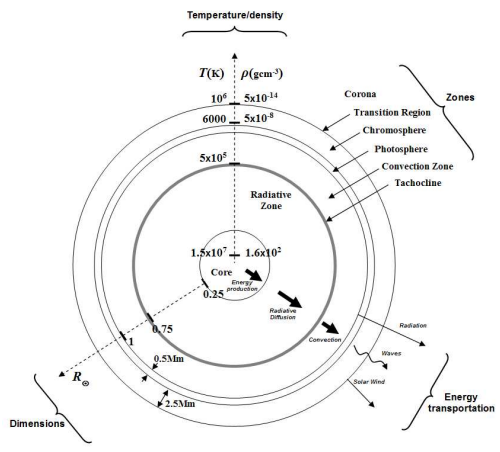
\includegraphics[width = 0.8\textwidth]{on}
\caption{Overview of the layers of the Sun. Source: https:$//$astroengine.files.wordpress.com$/$2012$/$07$/$thesis06.pdf.}
\label{fig_1}
\end{figure}
%T_regoins
\begin{figure}
\centering
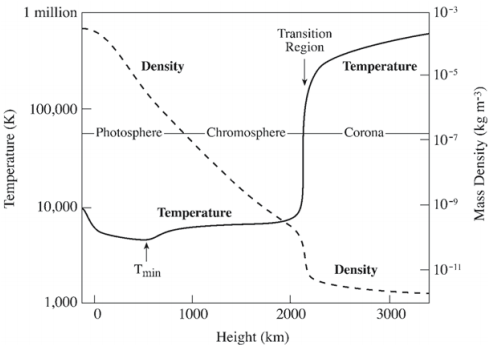
\includegraphics[width = 0.725\textwidth]{T_regoins}
\caption{Plot of the temperature and density from the photosphere to the corona. Plot taken from \cite{Lang_2006ses}.}
\label{fig_1a}
\end{figure}
%-------------------------
%\begin{figure}
%\centering
%\includegraphics[width = 0.85\textwidth]{sun_regions}
%\caption{Overview of the layers of the Sun. Source: http:$/ /$www.nasa.gov$/$mission$\_$pages$/$hinode$/$solar$\_ 020$.html.}
%\label{fig_1}
%\end{figure}
%-----------------------------------------
% 1 http://solarscience.msfc.nasa.gov/interior.shtml
% 2 http://www.nasa.gov/mission_pages/iris/multimedia/layerzoo.html
% Fig one: http://www.nasa.gov/mission_pages/hinode/solar_020.html
\subsection{Corona}
Above the chromosphere, the corona extends tens of million of kilometres into space. It is possible to see the corona with the naked eyes during eclipses as seen in fig. \ref{fig_2}. Otherwise to observe the corona a coronagraph is needed, which is a disk shaped instrument place on telescopes that can produce an artificial eclipse by blocking the light from the photosphere. The corona is continually expanding into interplanetary space by following the Sun's magnetic field lines, in this form it is referred to as the solar wind. The solar corona is the hot tenuous magnetised outer atmosphere of the Sun with an average temperature of $1-2$ MK, but can even reach $10$ MK. Despite its high temperature, it has a low amount of heat as it is very rarefied, with densities of the order of $10^{-12}$ kg m$^{-3}$ \citep{priest2014magnetohydrodynamics}. This in turn mean that the the energy density of the corona is much lower than that of the lower layers of the solar atmosphere, e.g. the photosphere where temperature is approximately $5000$ K. In spite of this the quiet Sun needs to have a constant energy input of $300$ W m$^2$ \citep{priest2014magnetohydrodynamics} to maintain observed coronal temperatures. \\ \\ The high temperature of the corona is evidenced by the presence of ions with many electrons removed from the atom. At high enough temperatures, atoms collide with one another with sufficient energy to free electrons. At very high temperatures, atoms such as iron is 9-13 times ionised. Fe X and Fe XIV occurs at temperatures of 1.3 $MK$ and 2.3  $MK$ respectively \citep{narayanan2014introduction}. The corona is typically observed in Extreme Ultraviolet (EUV) and X-rays due to its high temperatures (as seen in Fig. \ref{fig_2a}). \\ \\ Although the mechanism for transporting the energy from the photosphere upwards alludes us, it has widely been accepted that the solar magnetic field plays a major role. One key justification for this is to a first order approximation, the solar magnetic filed in the solar atmosphere extends vertically through the atmosphere connecting each layer together and thus, providing corridor for non-thermal energy transport. The magnetic field is thought to be generated in the tachocline (a shearing layer between the radiative and convection zone). The magnetic filed generate here are then convected up with the plasma to the photosphere, where it emerges and forms complex magnetic structure on various scales in the atmosphere (from Magnetic Bright Points (MBP) to coronal loops up to $100$ Mm). The Sun's magnetic field traps a majority of the plasma in the corona close to the star. These magnetic fields support waves oscillations which can be studies to in the coronal environment such as coronal loops which allows us to determine properties such as density \citep{Verwichte_2013A_A}, magnetic field strength \citep{Nakariakov_2001} and temperature \citep{De_Moortel_2003SoPh}.           
\begin{figure}
\centering
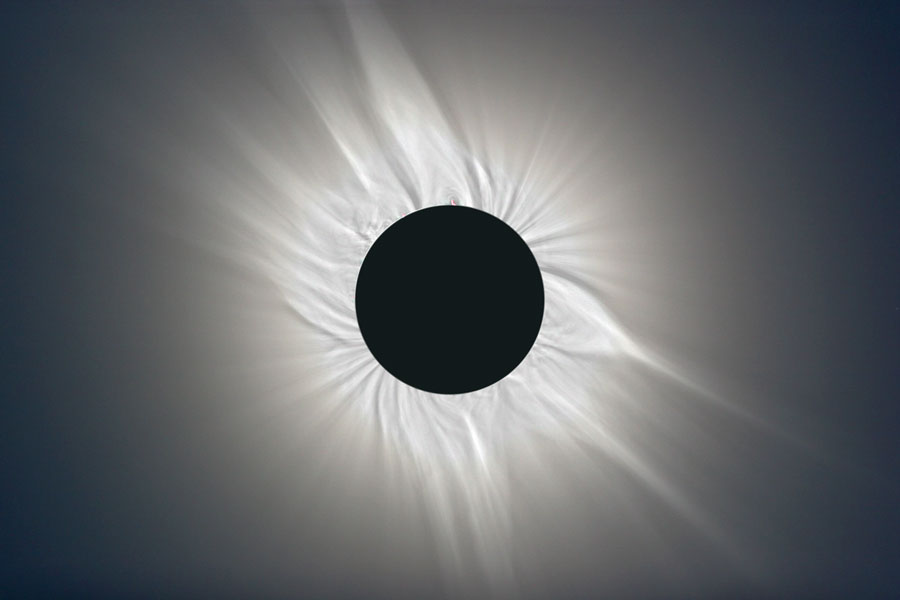
\includegraphics[width = 0.65\textwidth]{corona_vangorp}
\caption{Image of the Corona from a total eclipse that occurred on the March of 2006. Source: NASA APOD 26th of July 2009.}\label{fig_2}
\end{figure}
%% http:$//$apod.nasa.gov$/$apod$/$ap090726.html
\begin{figure}
\centering
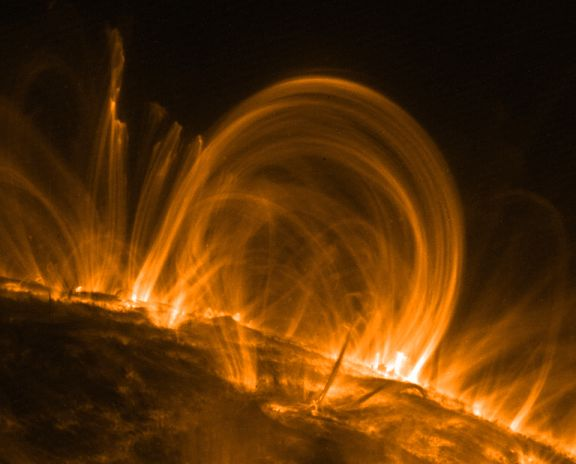
\includegraphics[width = 0.60\textwidth]{coronaloop_trace}
\caption{Image of a coronal loop in the Sun's atmosphere. This image was captured by TRACE in the UV at a wavelength of $171$\AA$ \ $ on Novermeber 6, 1999. Source: http:$//$www.nasa.gov$/$centers$/$goddard$/$news$/$topstory$/$2008$/$coronal$\_$loops.html}\label{fig_2a}
\end{figure}
%%loop_trace
\subsection{Solar Facts}
The values below are taken from \citep{priest2014magnetohydrodynamics}.  \\ \\
Age: $4.6 \times 10^9$ years. \\
Mass: $M_{\odot}= 1.99 \times 10^{30}$ kg. \\
Radius: $R_{\odot} = 6.96 \times 10^5$ km. \\
Surface temperature: $5785$ K. \\
Mean density: $1.4 \times 10^3$ kg m$^{-3}$. \\
Mean distance from Earth: $1$ AU = $1.5 \times 10^8$ km. \\
Surface gravity: $g_{0}=274$ m s$^-2$. \\
Equatorial Rotation Period: $26$ days. \\
Composition: $90 \%$ H, $10 \%$ He, $0.1 \%$ other elements.    
\subsection{Solar Jets}
The motivation for my work is to construct a model that accurately simulates waves in the Transition region. We are interested in spicules (solar jets) as these jets are ubiquitous ($100,000$  at  any  time \citep{Beckers1968}) on the Sun, thus are a good candidate for coronal heating. These jets could perturb the transition region (a thin region of approximately $100$ km between the chromosphere and corona where the temperature raises from $10^4$ K to $1$-$2$ MK) causing it to oscillate (akin to when a drum is struck). When a solar jet rises up from the photosphere to corona it will cause the Transition region to ripple and thus perturb the surrounding magnetic fields. The goal is to analyse the waves and the energy involved in these waves to investigate if they could significantly contribute to coronal heating. \\ \\ We will conduct numerical modelling research into the effects of spicules on the transition region, focusing on whether spicules are the drivers of TRQs \citep{Scullion2011}. TRQ are energetic waves in the transition region that evolves in a similar manner to waves on 2D elastic waveguides. To achieve this, we will construct a large sample of TRQ using IRIS and infer their properties both from imaging and spectral data. The discovery of a link between these waves and Rapid Blueshifted Excursions (RBE) identified in CRISP H-alpha data is potentially very far reaching. Work by \cite{Henriques2016} has already found convincing evidence of links between RBEs and coronal transient events, however, they did not study whether their coronal features corresponded to coherent waves (i.e. TRQ manifesting as propagating wave fronts). This task is vital for expanding our knowledge of the coupling between the lower solar atmosphere and the transition region. \\ \\ The importance of small-scale jets is well known as they are suggested to contribute to coronal heating and solar wind acceleration. Spicules themselves may be triggered by magnetic reconnection \citep{Pontieu2007} or waves \citep{DePontieu2004}. Although, it is currently unclear what the decisive physical factors that trigger spicules, reconnection and waves are both promising candidates for their contribution to the energy exchange between the the lower cool atmosphere and the corona. Meanwhile, apparent transverse motion within spicules and intermittent Doppler-shifts in coronal loops could be evidence in support of the existence of \Alfven or kink waves in the solar atmosphere. SP2RC has a method for constructing 3D MHD equilibrium for multiple magnetic flux tubes in a stratified solar atmosphere. This solar atmospheric model incorporates a wide and realistic range of scales. Taking advantage of a steady state for the background, the governing equations can be reduced, solving only the evolution for the perturbations if we choose to use the Sheffield Advance Code. Capturing the true dynamics of these phenomena requires realistic flux tube models and this is the aim of this project. We will study the jet origin, excitation and multiple jet excitation employing a novel 3D MHD code. We will validate results with high-resolution data (e.g. CRISP) to gain insight into the relationship between various solar transients (e.g. jets, MBPs, RBE). By using this combination of numerical simulations and observations of the penetration of jets from the chromosphere, through the transition region into the corona, we will reveal how momentum and energy are transported to the upper atmosphere. \\ \\
Observations have demonstrated the ubiquity of vortex motions present in the solar atmosphere. These are usually found at photospheric MBP groups. Previous MHD simulations have shown such vortices could be responsible for the generation of various types of MHD waves, yet their relationship with other ubiquitous transients-jets (spicules) is unclear.
\subsection{MHD Equations} 
We will model Solar jets by taking a fluid approach using the magnetohydrodynamic (MHD) equations. The MHD equations are a combination of the Navier$–$Stokes equations of fluid dynamics and  Maxwell's equations of electromagnetism. It describes the motion of magnetic fluids in the presence of the electromagnetic fields, which is well suited to describe the dynamics of a plasma. A plasma is a completely ionised gas, consisting of freely moving positively charged ions, which behaves collectively in the presence of a magnetic field and is the forth state of matter. From a human's perspective the typical states of matter encountered in our day to day life on Earth mainly appears in three phases of solid, liquid and gas. We may observe plasmas on Earth for example lightning, TVs and neon lamps. However, if we consider matter on a universal scale, then we see that $90 \%$ of baryonic matter in the universe is plasma. Hence, we conclude that plasma is the normal state of baryonic matter in the universe \citep{goedbloed2004principles}. An interesting property of the MHD equations is they are scale independent. This means the MHD equations provides a basis for the description of the macroscopic dynamics of $90 \%$ of baryonic matter in the Universe and also are applicable to laboratory plasma such as in tokamaks ($20$ m) to astrophysical plasmas such as accretion disc of a active galactic nucleus ($10^{21}$  m) \citep{goedbloed2004principles}. The MHD theory is a fluid approach which is valid if the length scales of the system are larger than the Debye shielding length. The Debye shielding length defines the typical length scale in which the ions and electrons neutralise one another and thus the particles feel no force from the electric field. The fluid motion describes the collective motion of particles. This collective interaction involving motion, currents and magnetic fields describes the general behaviour of the MHD fields. The MHD equations are given by the following:      
\begin{equation}\label{eq86}
\frac{\partial \rho}{\partial t} = - \nabla \cdot (\rho \boldsymbol{v}),
\end{equation}
\begin{equation}\label{eq87}
\rho \frac{d \boldsymbol{v}}{dt} = - \nabla p + \frac{1}{\mu_0} (\nabla \times \boldsymbol{B}) \times \boldsymbol{B} + \rho \boldsymbol{g},
\end{equation}
\begin{equation}\label{eq88}
\frac{dp}{dt} = - \gamma p \nabla \cdot \boldsymbol{v},
\end{equation}
\begin{equation}\label{eq89}
\frac{\partial \boldsymbol{B}}{\partial t} = \nabla \times (\boldsymbol{v} \times \boldsymbol{B}) - \frac{1}{\mu_0} \nabla \times (\eta \nabla \times \boldsymbol{B}),
\end{equation}
\begin{equation}\label{eq90}
\nabla \cdot \boldsymbol{B} = 0.
\end{equation}
Where Eq. (\ref{eq86}) is the mass continuity equation which states matter cannot be created or destroyed it simply changes to a different form of matter. Eq. (\ref{eq87}) is the momentum equation, it represents balance between acceleration, also the balance between the pressure gradient and the Lorentz force (force which is exerted by a magnetic field on a moving charge, $\frac{1}{\mu_0} (\nabla \times \boldsymbol{B}) \times \boldsymbol{B}$). As the Lorentz force is directed perpendicular to the magnetic field, this means that the acceleration along the magnetic field lines are caused by pressure gradient or gravity. Eq. \eqref{eq88} represents the internal energy and Eq. \eqref{eq89} is the induction equation and links the dynamics of the magnetic field through the velocity term. Eq. \eqref{eq90} is the solenoidal constraint and implies that there are no magnetic monopoles or pure sinks of the magnetic field.\\ \\ To gain intuitive understanding of oscillations in a plasma we derive analytically MHD equations. We take small perturbation with respect to the background quantities, therefore we define the following:
\begin{equation} \label{eq91}
\boldsymbol{B} = \boldsymbol{B}_0 + \boldsymbol{B}_1 (\boldsymbol{r},t) , \ \ \boldsymbol{v} = \boldsymbol{v}_1 (\boldsymbol{r}, t) , \ \ \rho = \rho_0 + \rho_1 ( \boldsymbol{r},t) , \ \ p = p_0 + p_1 ( \boldsymbol{r}, t) ,
\end{equation}
where $\boldsymbol{r} = (x,y,z)$ is the potion vector. The subscript $0$ ($1$) represents the equilibrium quantity (Eulerian perturbation). Where $v_0=0$ as we assume no background flow. Applying the perturbations shown by Eq. \eqref{eq91} to Eq. \eqref{eq86} to Eq. \eqref{eq90} obtains the linearised MHD equations: 
\begin{equation}
\frac{\partial \rho_1}{\partial t} = \nabla \cdot (\rho_0 \boldsymbol{v}_1) ,
\end{equation}
\begin{equation}
\rho_0 \frac{\partial \boldsymbol{v}_1}{\partial t}  = - \nabla p_1 + \frac{1}{\mu_0} (\nabla \times \boldsymbol{B}_0) \times \boldsymbol{B}_1 + \frac{1}{\mu_0} (\nabla \times \boldsymbol{B}_1) \times \boldsymbol{B}_0 ,
\end{equation}
\begin{equation}
\frac{\partial p_1}{\partial t} = - \boldsymbol{v}_1 \cdot \nabla p_0 - \gamma p_0 \nabla \cdot \boldsymbol{v}_1 , 
\end{equation}
\begin{equation}
\frac{\partial \boldsymbol{B}_1}{\partial t} = \nabla \times (\boldsymbol{v}_1 \times \boldsymbol{B}_0) - \nabla \times (\eta \nabla \times \boldsymbol{B}_1) ,
\end{equation}
\begin{equation}
\nabla \cdot \boldsymbol{B}_0 = \nabla \cdot \boldsymbol{B}_1 = 0 .
\end{equation}
These equations are the used to construct our models for the oscillations. 
\subsection{\Alfven Waves}\label{c2}
To define magnetic waves, we take the linearised ideal MHD equations with no gravity ($\boldsymbol{g}=0$) and a uniform magnetic field in the $z$ direction ($\boldsymbol{B_0}=B_0 \boldsymbol{\hat{z}}$). We assume the diffusion term is $\eta=0$ and we take a pressureless ($p_0=p_1=0$) plasma with no density variations ($\rho_1=0$). This allows us to see the effect of the magnetic field on waves and thus the basic properties of an \Alfven wave. We look for plane waves and Fourier analyse by assuming the perturbed parameters are of the form:  
\begin{equation}
\boldsymbol{v_1} = \boldsymbol{C_{v}} \exp(i(\boldsymbol{k} \cdot \boldsymbol{r}- \omega t)),
\end{equation}
where $\boldsymbol{k} = (k_x,k_y,k_z)$ is the wave vector, $\boldsymbol{r} = (x,y,z)$ is the position vector and $\omega$ is the frequency. With above assumptions the linearised MHD equations become:
\begin{equation}\label{n31}
i \boldsymbol{k} \cdot \boldsymbol{v} = 0,
\end{equation}
\begin{equation}\label{n32}
- \rho_0 i \omega \boldsymbol{v_1} = \frac{1}{\mu_0} (i \boldsymbol{k} \times \boldsymbol{B_1}) \times \boldsymbol{B_0},
\end{equation}
\begin{equation}\label{n33}
-i \omega \boldsymbol{B_1} = i \boldsymbol{k} \times (\boldsymbol{v_1} \times \boldsymbol{B_0}),
\end{equation}
\begin{equation}\label{n34}
i \boldsymbol{k} \cdot \boldsymbol{B_0} = i \boldsymbol{k} \cdot \boldsymbol{B_1} = 0.
\end{equation}
Before solving for the dispersion relation, we look for some further characteristics of the magnetic wave. We can see straight away from Eq. (\ref{n31}) that \Alfven waves are incompressible. By taking (\ref{n32})$\cdot \boldsymbol{B_0}$ we obtain:
\begin{equation}\label{n35}
\boldsymbol{v_1} \cdot \boldsymbol{B_0} = 0,
\end{equation}
Eq. (\ref{n35}) shows the motion is perpendicular to the equilibrium magnetic field and therefore \Alfven waves are transverse waves. Next taking equation (\ref{n33})$\cdot B_0$ it can be shown:
\begin{equation}\label{n36}
\boldsymbol{B_1} \cdot \boldsymbol{B_0} = 0.
\end{equation}     
Eq. (\ref{n36}) proves that the perturbation of the magnetic field is perpendicular to the equilibrium magnetic field. Lastly to obtain the frequency for the \Alfven waves ($\omega_A$) we multiply Eq. (\ref{n33}) by $\omega$ and substitute into the equation of motion (\ref{n32}), which yields:
\begin{equation}
i \omega^2 \boldsymbol{B_1} = \frac{1}{\mu_0 \rho_0} i k \left[ ( (\boldsymbol{B}_0 \cdot \boldsymbol{k}) \boldsymbol{B}_1 - (\boldsymbol{B}_1 \cdot \boldsymbol{B}_0) \boldsymbol{k})\times \boldsymbol{B}_0 \right] .
\end{equation}   
Using Eq. \eqref{n36} and Eq. \eqref{n34} we can obtain:
\begin{equation}\label{n29}
\omega_A = \pm k_z V_A = \pm V_A \cos(\theta),
\end{equation}  
where:
\begin{equation} \label{eq93}
V_A= \frac{B_0}{\sqrt{\mu_0 \rho_0}}, 
\end{equation}
is the \Alfven speed. Eq. (\ref{n29}) shows that \Alfven waves are anisotropic as they propagate in a preferred direction relative to the equilibrium magnetic field. This anisotropic behaviour is clearly seen in the phase diagram given by fig. \ref{fig_9}. Their group speed is calculated as follows:
\begin{equation}
\boldsymbol{V}_{g,A} = \frac{\partial \omega_A}{\partial \boldsymbol{k}} = \pm V_A \boldsymbol{\hat{z}}. 
\end{equation}  
As the group speed is in the same direction as the equilibrium magnetic field, it is deduced that energy is transmitted only along the magnetic field line at the \Alfven speed. 
\subsection{Magnetoacoustic Waves} 
Taking the same assumptions as outlined in the beginning of chapter \ref{c2}, except this time including pressure and the density variation, the MHD equations become: 
\begin{equation}\label{n41}
-i \omega \rho_1+ \rho_0 i \boldsymbol{k} \cdot \boldsymbol{v_1} = 0,
\end{equation}
\begin{equation}\label{n37}
- \rho_0 i \omega \boldsymbol{v} = \frac{1}{\mu_0} (i \boldsymbol{k} \times \boldsymbol{B_1}) \times \boldsymbol{B_0}-i \boldsymbol{k} p_1,
\end{equation}
\begin{equation}\label{n38}
- \rho_0 i \omega \boldsymbol{v_1} = \frac{1}{\mu_0} (i \boldsymbol{k} \times \boldsymbol{B_1}) \times \boldsymbol{B_0},
\end{equation}
\begin{equation}\label{n42}
-i \omega p_1 = - \gamma p_0 i \boldsymbol{k} \cdot \boldsymbol{v_1},
\end{equation}
\begin{equation}\label{n39}
-i \omega \boldsymbol{B_1} = i \boldsymbol{k} \times (\boldsymbol{v_1} \times \boldsymbol{B_0}),
\end{equation}
\begin{equation}\label{n40}
i \boldsymbol{k} \cdot \boldsymbol{B_1} = 0.
\end{equation}
Starting with the equation of motion (\ref{n38}) and applying equations (\ref{n39}),(\ref{n36}) and (\ref{n40}), one can acquire the following dispersion relation: 
\begin{equation}
 \omega^4-k^2\omega^2(C_s^2+V_A^2)+k^2 C^2_s V^2_A k^2_z = 0,
\end{equation} 
where $C_s=\sqrt{\frac{\gamma p_0}{\rho_0}}$ is the sound speed. The roots to this dispersion relation are: 
\begin{equation}\label{n30}
\omega_s,f = \frac{k^2}{2} \left[ C_s^2+V^2_A \pm \sqrt{(C^2_s+V^2_A)^2-4C^2_s V^2_A \cos^2(\theta)} \right] .
\end{equation}
Eq.(\ref{n29}) yields the frequency for \Alfven waves ($\omega_A$) and Eq. (\ref{n30}) gives the frequency for the fast ($\omega_f$ for $+$) and slow ($\omega_s$ for $-$) magnetoacoustic (MA) waves. The phase speed diagram is shown in Fig. \ref{fig_9}. We can see from Eq. (\ref{n30}) that the fast MA wave is in phase with the pressure and magnetic pressure, while the slow MA waves is out of phase with the  pressure and magnetic pressure. The MA waves are compressive modes. Perturbation of the velocity and the magnetic field remain in the plane defined by the magnetic field and the wave normal. From the phase diagram when the waves are propagating perpendicular to the magnetic field then $\omega_s / \boldsymbol{k}=0$ and $\omega_f / \boldsymbol{k} = (V_A^2+C_s^2)^{1/2}$. This shows the waves degenerate to MA mode as this is the only mode that propagates with a nonvanishing speed at $\theta=90^{\circ}$. If the propagation is parallel to $B_0$, $\omega_f / \boldsymbol{k}=V_A$. From the group velocity diagram (see Fig. \ref{fig_15}) we see that the energy travels fastest across the magnetic field line for the fast MA wave. The slow MA wave energy transport along the magnetic field line is restricted to a cusp shape along $B_0$. We see that the \Alfven group velocity remains purely parallel to the equilibrium magnetic field.
%-------------------------------------------         
\begin{figure}[h]
\centering
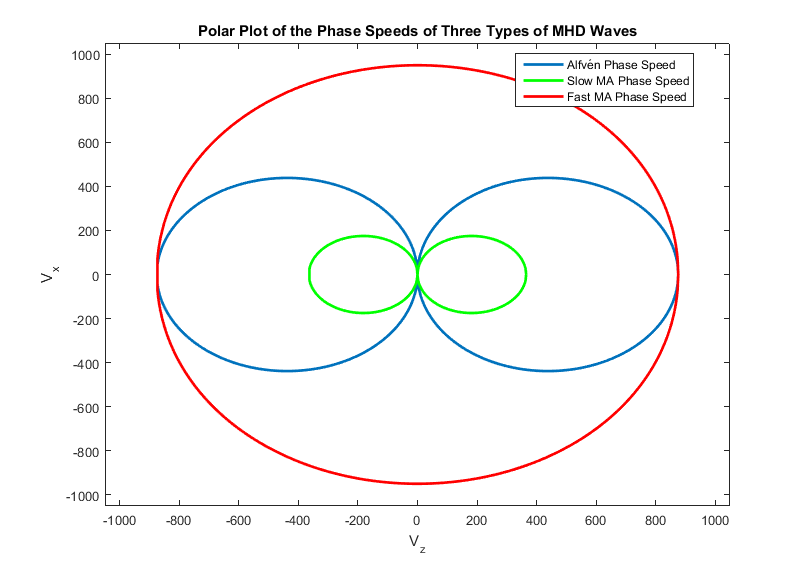
\includegraphics[width = 0.70\textwidth]{disp_sq}
\caption{Phase diagram of the \Alfven wave (blue), fast MA wave (red) and slow MA wave (green). The equilibrium magnetic field is taken in the $z$-direction. This diagram corresponds to typical coronal values with $V_A=876$ $km/s$ and $C_s = 365$ $km/s$. This figure was plotted using my own code in MATLAB.}\label{fig_9} 
\end{figure}
%---------------------------
\begin{figure}[h]
\centering
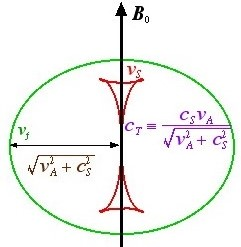
\includegraphics[width = 0.35\textwidth]{dispersion_g}
\caption{Group velocity diagram of the fast MA wave (green) and slow MA wave (red). Source: http:$/ /$solar.physics.montana.edu$/$magara$/$Research$/$Topics$/$MHD$\_$waves$/$mhdw.html .}\label{fig_15} 
\end{figure}
\newpage
%--------------------------
% find group velocity diagram

\subsection{Coronal Heating} \label{sec1}
The coronal heating problem has puzzled scientist for over the last 70 years. In this thesis we investigate one of the possible mechanisms for which the wave energy in the \Alfven waves can be dissipated into heat. There are 2 main candidates for heating the solar corona. The first one is related to flares. Such phenomena involve large scale magnetic to thermal energy conversion in a process known as magnetic reconnection, however these are not frequent enough to heat the entire solar corona. A leading theory for explaining the solar corona is based on this mechanism, but at much smaller energetic scales known as ``nanoflare" theory. This theory implies that reconnection may be occurring everywhere in the corona, leading to energy release in spatial locations too small to be detected observationally but frequent enough to be effective and heat the corona \citep{Narain_2006JApA}. Another of the hypothesised explanation to the coronal heating problem is based on wave heating. One of the main candidates for heating the corona is the \Alfven wave which carry the required energy to sufficiently heat the corona \citep{Aschwanden_2005_psci}. However, \Alfven waves are very difficult to dissipate in homogeneous regions in the corona as \Alfven waves are shear waves and the coronal shear viscosity is very low \citep{Hollweg_1991_mcch}. Therefore we need a mechanism to dissipate the energy carried by the \Alfven waves to heat the plasma. \\ \\ The nature of the process that heats the corona and the acceleration of the solar wind remains a major challenge in solar physics currently \citep{narayanan2014introduction}. Convection and conduction are unable to transport the energy due to the low density. Radiation can not possibility due to the optical depth being too high also because of the low density. While regions in the chromosphere have more complex thermal characteristics, this does not hold true for the corona. Therefore other energy transport mechanisms have to be heating the solar atmosphere, from the low chromosphere, to the corona.\\ \\ In \cite{Heyvaerts_1983_A} they came to the conclusion that phase mixing is a likely mechanisms to dissipate shear \Alfven waves in solar corona loops. Phase mixing occurs when the local \Alfven speed varies with position for example if the density was inhomogeneous (a condition typically encountered in the sun's atmosphere). \Alfven waves of the same frequencies on different field lines travel with different speeds and therefore will have different wavenumbers. The wave oscillations of neighbouring field lines are subjected to friction from kinematic and shear viscosity because they have marginally differing phase speeds \citep{Aschwanden_2005_psci}. If we take a standing \Alfven wave in closed field region as seen in Fig. \ref{fig_13}, the \Alfven wavenumber is fixed by the finite size of the region. As the atmosphere is inhomogeneous, the \Alfven velocity will make the frequency of the wave have positional dependence:
\begin{equation}
\omega(x) = V_A(x)k ,
\end{equation}     
for the wave number $k=2 \pi n / L$, where $L$ is the loop length. From \cite{Hood_1997_A} it is stated that in a non-dissipative plasma, linear \Alfven waves of wavenumber $k$ have solution $V \sim \exp(i \omega(x)t-ikz)$, which implies:
\begin{equation}\label{eq49}
\frac{\partial V}{\partial x} \sim Vt \omega^{\prime} (x).
\end{equation}
Eq. (\ref{eq49}) shows the gradients in the x-direction increases with time and this leads to the waves becoming phased mixed as they propagate. As each field has initially its own phase speed, as waves evolves their motion will move out of phase with respect to neighbouring field lines. This makes large velocity gradients across the loop and small length scales are created which allow for dissipation to have a large effect.        
%----------------------------------------------
\begin{figure}[h]
\centering
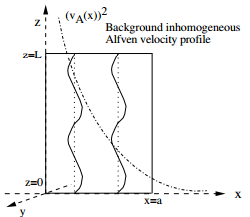
\includegraphics[width = 0.6\textwidth]{phase_mix}
\caption{ Model of phase mixing in coronal loop. Figure from \cite{Hood_1997_A}.}
\label{fig_13}
\end{figure}
However, when gravitational stratification of the solar corona is included in the calculations, phase mixing becomes a less effective mechanism for dissipation \citep{De_Moortel_1999_A}. The effects of phase mixing is moved to lower altitudes if curvature of the solar corona is taken into account \citep{De_Moortel_2000_A}.           
\\ \\ Another mechanism is resonant absorption. A necessary condition for the resonance between these two waves to take place is that they must travel at the same speed. While the speed of global kink wave is fixed, the speed of the \Alfven wave changes depending on the local density. In the case of a coronal loop, we have the density belonging to the structure is greater than the ambient plasma surrounding, thus the \Alfven speed will increase as you move from the internal to external region (see Fig. \ref{fig_3_1}). Resonant absorption creates a thin resonant layer localised around the boundary of the tube where the density is inhomogeneous and the phase speeds of the kink waves matches the external \Alfven waves phase speed. In this resonant layer, the kink waves (which displays a predominantly transverse motion) is converted into an azimuthal motion as it resonates with the torsional \Alfven wave. This is sometimes compared to a dancer skirt where the dancer's hips move side to side (representing the transverse motions of the coronal loop) results in rotational motions of the skirt (representing the resonance flow, see Fig. \ref{fig_14}). The azimuthal motions of the torsional \Alfven waves are amplified and create velocity shear. This configuration leads to Kelvin$-$Helmholtz instability (KHI) as seen in Fig. \ref{fig_14}, creating turbulence at the loop edges which causes dissipation of the wave energy into heat \citep{Antolin_2015b}. Resonant absorption is effectively damps the kink oscillations. In this thesis we will include the effect of resonant absorption in our model in an analytical manner. While resonant absorption is theoretically sound mechanism for damping kink waves and producing heat in the corona, it lacks sufficient direct observational evidence \citep{Antolin_2015a}. One of the goals of this thesis is to include the effects of resonant absorption in our models. This is a step towards obtaining the plasma parameters which can be used make synthetic observations and possibly identify observational features of resonant absorption.                      
%---------------------------------------------
\begin{figure}[h]
\centering
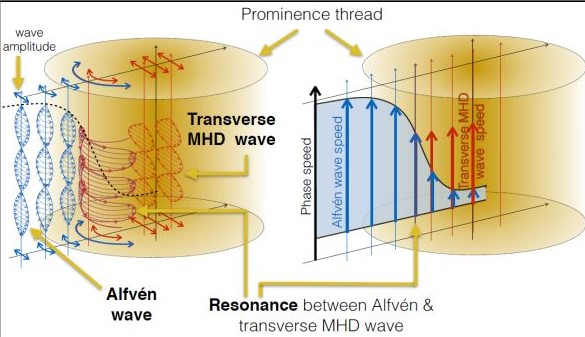
\includegraphics[width = 0.8\textwidth]{fig7el_s}
\caption{  The tube on the left shows resonant absorption between \Alfven waves in blue and kink waves (also know as transverse MHD wave) in red. It depicts the transverse motions being converted to azimuthal motions near the loop boundary. The tube to the right shows the radial profile of the \Alfven wave phase speed. Source:  http:$//$hinode.nao.ac.jp$/$news$/$1508Hinode-IRIS$/$long.shtml.}
\label{fig_3_1}
\end{figure} 
%---------------------------------------------
\begin{figure}[h]
\centering
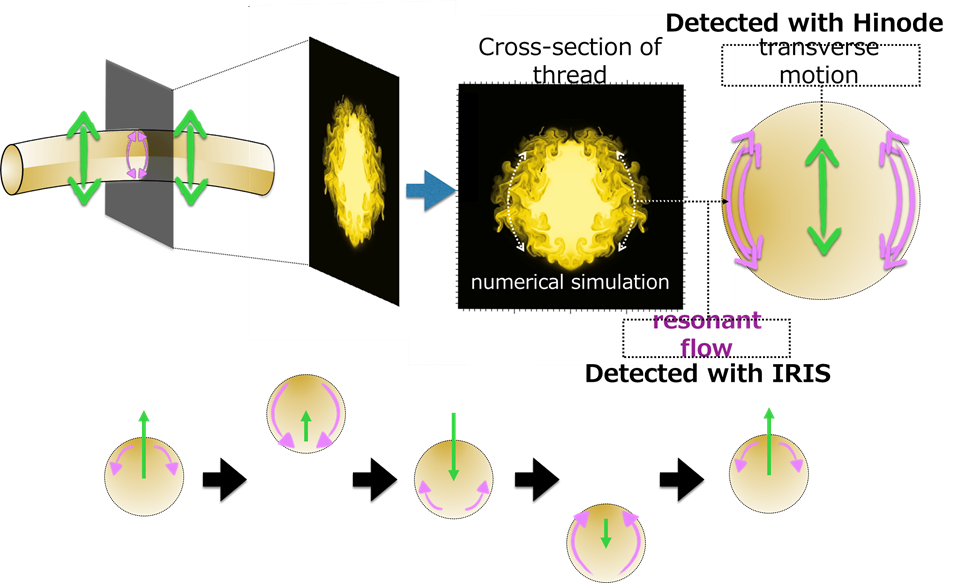
\includegraphics[width = 0.7\textwidth]{res_abs_mot}
\caption{The evolution of the cross section of a flux tube is shown. The kink waves' transverse oscillations are known by the green arrows. The resonance between the kink wave and \Alfven wave produces an azimuthal resonance flow given by the purple arrows, this leads to KHI. Source: http:$//$hinode.nao.ac.jp$/$news$/$1508Hinode-IRIS$/$long.shtml. }
\label{fig_14}
\end{figure} 
\subsection{MPI-AMRVAC}
MPI-AMRVAC is an MPI-parallelized Adaptive Mesh Refinement code. AMRVAC solves a systems of hyperbolic partial differential equations by a number of different numerical schemes. In principle the ARMVAC handles anything of the generic form: 
\begin{equation}
\frac{\partial \boldsymbol{U}}{\partial t} + \nabla \cdot \boldsymbol{F}(\boldsymbol{U}) = \boldsymbol{S}_{phys} (\boldsymbol{U}, \partial_{i} \boldsymbol{U}, \partial_i \partial_j \boldsymbol{U},\boldsymbol{x},t) .
\end{equation}
%solves the MHD equations in the following form:
%\begin{equation}
%\frac{\partial \rho}{\partial t} + \nabla \cdot (\boldsymbol{v} \rho) = 0 ,
%\end{equation}
%\begin{equation}
%\frac{\partial \rho \boldsymbol{v}}{\partial t} + \nabla \cdot (\boldsymbol{v} \rho \boldsymbol{v} - \boldsymbol{BB})+ \nabla p_{tot} = 0 ,
%\end{equation}
%\begin{equation}
%\frac{\partial e}{\partial t} + \nabla \cdot (\boldsymbol{v}e - \boldsymbol{BB} \cdot + \boldsymbol{v} p_tot) = \nabla \cdot (\boldsymbol{B} \times \eta \boldsymbol{j}) ,
%\end{equation}
%\begin{equation}
%\frac{\partial \boldsymbol{B}}{\partial t}+ \nabla \cdot (\boldsymbol{Bv}-\boldsymbol{Bv}) = -\nabla \times (\eta \boldsymbol{j}) ,
%\end{equation}
%\begin{equation}
%p=(\gamma-1)(e- \frac{\rho \boldsymbol{v}^2-\boldsymbol{B}^2}{2}) .
%\end{equation}
The main focus of this software is on conservation laws in particular with shock dominated problems. AMRVAC has been constructed so it is a single versatile software with options and switches for various problems (e.g. HD, MHD, adiabatic, relativistic, choices in numerical solvers, ect) rather than developing a different method or version for each problem separately. The advantage of this approach is that it allows for a reduction of overall time for software development. One of the main reasons for using AMRVAC for carrying out numerical simulations of these jets is to deal with differences in the order of magnitude in length scales involved in this research.
\subsubsection{Numerical Techniques}
Solving differential equations are key part of understanding the physics occurring in nature. Often coupled systems of differential equations can not be solved analytically without making major assumption to simply the equation and thus removing important physics from the original problem. A classic example of a system of equations which isn't solvable analytically is the three body problem where using Newtonian mechanics you consider three masses interacting with one another through gravitational force. The numerical soultions to this problem allowed the revolution in modern space flights, and the launch of the two Voyager probes. By using numerical techniques on the MHD equations we gain an insight into systems which are too complex to obtain analytically.  \\ \\A differential is the gradient of a function over an infinitesimally small range. The numerical approximation takes this range and makes it finite, calculation the differential from an approximation dependent on the selected method. In the sub-sections I will summarise a selection of solvers used in the MPI-AMRVAC code that are applied in this thesis.
\subsubsection{Finite Difference Method}
The general expression for a derivative is the following:
\begin{equation}
f'(x)=\lim\limits _{h\to0}\frac{f(x+h)-f(x)}{h} , 
\end{equation}
the finite difference method (FDM) approximates this equation by taking the step size $h$ as finite. The general form of a finite difference equation is $f(x+b)-f(x+a)$. The two simplest forms are:
\begin{align}
\Delta_+ f =  f(x+h)-f(x), \\
\Delta_- f = f(x-h)-f(x) .
\end{align}
These equations can be used to calculate the derivatives by using the following:
\begin{align}
\text{Forward Difference: }&f'(x) = \frac{f(x+h)-f(h)}{h} , \\
\text{Backwards Difference: }&f'(x) = \frac{f(x)-f(x-h)}{h}
\end{align}
These equations can be derived from a Taylor expansion of $f(x\pm h)$,
\begin{align}
f(x-h) & = f(x)-h f'(x)+\frac{h^{2}f''(x)}{2!}-\frac{h^{3}f'''(x)}{3!}+\frac{h^{4}f^{iv}(x)}{4!}+...\label{eq:TaylorForward}\\
f(x+h) & = f(x)+h f'(x)+\frac{h^{2}f''(x)}{2!}+\frac{h^{3}f'''(x)}{3!}+\frac{h^{4}f^{iv}(x)}{4!}+...\label{eq:TaylorBackward}
\end{align}
The forward (backwards) difference equations is the first-order truncation of the $f(x+h)$ ($f(x+h)$) Taylor series. From this it can be seen that the truncation error of a forward and backward difference approximation is $O(h)$, and that the accuracy is easily improved by increasing the number of terms included. \\ \\
Another variation of FDM that reduces the error, while maintaining the first-order nature of these solutions is achieved by combining the forward and backward difference into a central difference approximation of the following form: 
\begin{equation}
f(x)=\frac{1}{2} \left(f(x + h) + f(x - h)\right).
\end{equation}
Preforming a Taylor expansion and taking first order as previous done results in the following: 
\begin{equation}
f'(x)=\frac{f(x+h)-f(x-h)}{2h}.\label{eq:First Order CD}
\end{equation}
The  error for central difference approximation $O(h^{2})$ as we have combined both the two Taylor series expansions. The accuracy of the solution is important, for it determines how well the computed solution represents the true solution. The most obvious way to increase the accuracy of the solution is to increase the number of terms included from the Taylor expansion of the forward and backward differences. For example the derivation of a fourth-order central difference scheme which can be calculated by starting from Eqs. \eqref{eq:TaylorForward}-\eqref{eq:TaylorBackward} and subtracting the second from the first, to the fourth order gives, in one dimension the following:
\begin{equation}
f(x+h)-f(x-h)=2 h f'(x)+\frac{2 h^{3} f'''(x)}{3!}+O(h^{4}).\label{eq:centraldifferencedx}
\end{equation}
The next step is to calculate the same subtraction for $2 h$ which can be written as:
\begin{equation}
f(x+2 h)-f(x-2 h)=4 h f'(x)+\frac{16 h^{3}f'''(x)}{3!}+O(h^{4}).\label{eq:CentralDifference2dx}
\end{equation}
Then subtracting \eqref{eq:CentralDifference2dx} from $8\times$(\eqref{eq:centraldifferencedx}) and rearranging for $f'(x)$ results in:
\begin{equation}
f'(x)=\frac{8f(x+h)-8f(x-h)-f(x+2h)+f(x-2h)}{12h}+O(h^{4}),\label{eq:4thOrderCentralDifferenceUniform}
\end{equation}
which is the fourth order central difference scheme in one dimension for a uniform spacing of $\pm h$.
This scheme can be expanded into $n$ dimensions by using the basic property of differentiation $\frac{\partial^{2}u}{\partial x\partial y}=\frac{\partial}{\partial x}\left(\frac{\partial u}{\partial y}\right)=\frac{\partial}{\partial y}\left(\frac{\partial u}{\partial x}\right)$. This scheme provides good accuracy while being computationally efficient.
\subsubsection{TVLD}
\newpage
\bibliographystyle{aasjournal}
\bibliography{lit_bib}
\addcontentsline{toc}{chapter}{Bibliography}
\newpage


\end{document}